\documentclass{standalone}
\usepackage{tikz}
\begin{document}
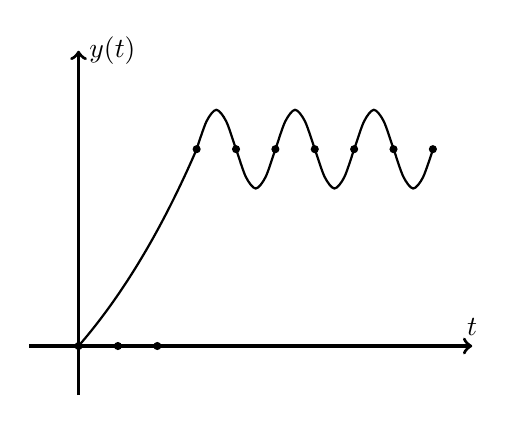
\begin{tikzpicture}[scale=2.5]
    \draw[->,very thick](-0.25,0)--(2,0)node[above]{$t$};
    \draw[->,very thick](0,-0.25)--(0,1.5)node[right]{$y(t)$};

    \draw[-,thick]plot[smooth, domain=0:0.6](\x,{3.174^(\x)-1});
    \draw[-,thick]plot[smooth, domain=0.6:1.8](\x,{1+0.2*sin(15.7*((\x)-0.6) r)});

    \filldraw[black](0,0)circle(0.5pt);
    \filldraw[black](0.2,0)circle(0.5pt);
    \filldraw[black](0.4,0)circle(0.5pt);
    \filldraw[black](0.6,1)circle(0.5pt);
    \filldraw[black](0.8,1)circle(0.5pt);
    \filldraw[black](1,1)circle(0.5pt);
    \filldraw[black](1.2,1)circle(0.5pt);
    \filldraw[black](1.4,1)circle(0.5pt);
    \filldraw[black](1.6,1)circle(0.5pt);
    \filldraw[black](1.8,1)circle(0.5pt);
\end{tikzpicture}
\end{document}